\documentclass{standalone}
\usepackage{tikz}
\usetikzlibrary{backgrounds}
\begin{document}
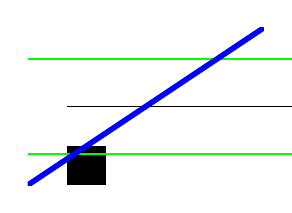
\begin{tikzpicture}
  \begin{scope}[blue, line width=2pt]
    \clip (0,0) rectangle (3,2);
    \draw (0,0) -- (3,2);
    % The scope's red and the enclosing blue are not used on the layer; the key's green is.
    \begin{scope}[on background layer, red, xshift=0.5cm]
      \draw (0,1) -- (3,1);
      \fill (0,0) rectangle (0.5,0.5);
    \end{scope}
    \begin{scope}[on background layer={green, thick}]
      \draw (0,0.4) -- (4,0.4);
    \end{scope}
    % The same with the environment.
    \begin{pgfonlayer}{background}
      \begin{scope}[green, thick]
        \draw (0,1.6) -- (4,1.6);
      \end{scope}
    \end{pgfonlayer}
  \end{scope}
\end{tikzpicture}
\end{document}
